\documentclass[draft]{article}
\usepackage[utf8]{inputenc}
\usepackage[dvips]{graphicx, color}

\usepackage{hevea}

% for hevea
\usepackage{fancysection}
\newcommand{\heveaimagedir}{image}

% lstlisting
\usepackage{listings}

\lstdefinestyle{shell}{%
  keywordstyle={\color{blue}},%
  stringstyle={\color{magenta}},%
  commentstyle={\em\color{magenta}}}

\lstnewenvironment{code}
  {\setenvclass{lstlisting}{code}\lstset{%
      language=Lisp,%
      keywordstyle={\color{blue}},%
      stringstyle={\color{magenta}},%
      morekeywords={define,class,-,method,new}}}
  {}

\lstnewenvironment{cmd}
  {\setenvclass{lstlisting}{cmd}\lstset{}}
  {}

\lstnewenvironment{bnf}
  {\setenvclass{lstlisting}{bnf}\lstset{%
      keywordstyle={\bf},%
      morekeywords={:=}%
  }}
  {}

\newstyle{.code}{font-family:monospace;white-space:pre;
border-left:solid black;padding-left:2ex;margin-left:2ex;}
\newstyle{.cmd}{font-family:monospace;white-space:pre;
border-left:solid black;padding-left:2ex;margin-left:2ex;}

\begin{document}
\title{SchemeABC Reference 0.5.0}
\author{MIZUNO Hiroki}
\date{2009/05/27}
\maketitle
\tableofcontents

\section{Quick Start}
\subsection{動作環境}

ビルドには以下の環境が必要です。
\begin{itemize}
\item \footahref{http://caml.inria.fr/}{OCaml 3.11}以降
\item \footahref{http://www.camlcity.org/archive/programming/findlib.html}{Findlib}
\item \footahref{http://omake.metaprl.org/}{omake}
\item cpp
\end{itemize}

また以下のライブラリが必要になります。
\begin{itemize}
\item \footahref{http://code.google.com/p/ocaml-extlib/}{extlib}
\item \footahref{http://tech.motion-twin.com/xmllight.html}{xml-light}
\item \footahref{http://www.xs4all.nl/~mmzeeman/ocaml/ounit-doc/OUnit.html}{OUnit}
\end{itemize}

動作時には以下のソフトウェアが必要です。
\begin{itemize}
\item m4
\item \footahref{http://swfmill.org/}{swfmill}(svn trunk版)
\end{itemize}

開発は以下のプラットフォームで行なっています。Windowsでも動作することを目指していますが、現状ではいくつかの点で不安定です。
\begin{itemize}
\item MacOS X 10.5.7
\item Ubuntu 9.04
\end{itemize}


\subsection{ビルド方法}
一般的なシステムの場合、以下のコマンドでインストールが可能です。
\begin{cmd}
$ omake config
$ omake all
$ sudo omake install
\end{cmd} % $

インストール先のディレクトリを変更したい場合は、\verb!omake config!で指定します。

\begin{cmd}
$ omake config PREFIX=/path/to
\end{cmd} % $

\verb!PREFIX!以外にも表\ref{option}に示すオプションが利用可能です。

\begin{table}
\centering
\caption{利用可能なオプション}\label{option}
\begin{tabular}{|l|l|l|}
\hline
オプション名     & 説明 & デフォルト値 \\\hline
\verb!PREFIX!    & インストール先ディレクトリ & /usr/local \\
\verb!LIB_DIR!   & ライブラリのインストール先 & \verb!$PREFIX/lib/habc! \\
\verb!SHARE_DIR! & 共有ファイルのインストール先 & \verb!$PREFIX/share/habc! \\
\verb!BIN_DIR!   & コマンドのインストール先     & \verb!$PREFIX/bin! \\
\hline
\end{tabular}
\end{table}

\subsection{Hello,world}

``Hello,world''を表示するプログラムは以下のようになります。
\begin{code}
(define-class Main (flash.display.Sprite) ())

(define-method init ([self Main])
  (let [(t (new flash.text.TextField))]
    (appendText t "Hello,world!!")
    (addChild   self t)))
\end{code}

これをビルドします。
\begin{cmd}
$ habc --height=100 --width=100 -o hello example/swf.scm
\end{cmd} % $

生成された\verb!hello.swf!を適当なブラウザで開くと、図\ref{hello}が表示されます。

\begin{figure}
\centering
%BEGIN IMAGE
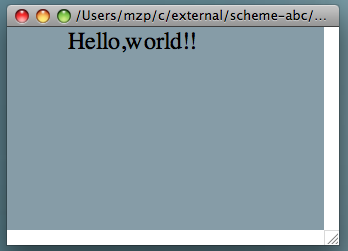
\includegraphics{hello}
%END IMAGE
%HEVEA \imageflush
\caption{Hello}\label{hello}
\end{figure}

\section{式}
\subsection{値}
\subsubsection{整数}

\begin{bnf}
int :=  (+ | - )? (oct | hex)
oct :=  [0-9]+
hex :=  "0x" [0-9A-Fa-f]+
\end{bnf}

整数値としては、10進整数値と16進整数値が利用可能です。

10進整数値は\verb!42!のような形をしています。また、\verb!-42!のように負の数も書けます。

16進整数値は\verb!0x1F!のように\verb!0x!で始まる必要があります。

\subsubsection{浮動小数}
\begin{bnf}
float :=  (+ | - )? [0-9]+ "." [0-9]+
\end{bnf}

浮動小数は、\verb!10.42!のような形をしています。\verb!42.!のように\verb!.!の後のを省略することはできません。

\subsubsection{真偽値}


\subsubsection{文字列}

\subsection{手続き}
\subsubsection{lambda}
\subsubsection{呼び出し}

\subsection{変数束縛}
\subsubsection{let}
\subsubsection{letrec}
\subsubsection{参照}

\subsection{条件分岐}
\subsubsection{if}
\subsubsection{cond}

\subsection{逐次実行}
\subsubsection{begin}

\section{文}
\subsection{式}

\subsection{define}

\section{オブジェクトシステム}
CLOSライクです。

\section{標準ライブラリ}
まだありません。

\section{コマンドラインオプション}

\section{ライセンス}
\verb!pa_oo.ml! is written by \footahref{http://www.math.nagoya-u.ac.jp/~garrigue/code/ocaml.html}{Jacques Garrigue.} and modified by
\footahref{http://d.hatena.ne.jp/osiire/}{OGASAWARA Satoshi.}, license is BSD.

\verb!pa_openin.ml! is written by \footahref{http://d.hatena.ne.jp/osiire/}{Alain Frisch.}, licence is Public Domain.

Other codes is written by \footahref{http://happyabc.org}{MIZUNO Hiroki.}, licence is MIT Licence.

\end{document}
